\section{Announcements}

\begin{frame}{Announcement 1: Modification on Class Schedule}
  There was an extension for Grade submission in the graduate school, so
  I have revised the class schedule and deadlines:\bigskip

  \begin{itemize}
    \item 6/19 -- Topic 8: Multiple Comparisons
    \item 6/26 -- Topic 7: Sample Sizes
    \item 6/27 -- (Saturday) Cancelled
    \item 7/3  -- Open Question Session
    \item 7/20 -- Report 3 submission Deadline
    \item 7/26 -- Grades Announcement
  \end{itemize}
\end{frame}

\begin{frame}{Announcement 2: Third Report and Grading}

  {\smaller
  \begin{block}{Third Report Topic}
    Like the first and second report, in the third report you have to design, run and analyse an experiment.\bigskip

    For report 3, you must include in your experiment design:
    \begin{itemize}
      \item Calculation of sample sizes (next lecture);
      \item Comparison of multiple samples (this lecture);
    \end{itemize}
  \end{block}
  \begin{exampleblock}{Grading}
    Originally, I was expecting to have some extra time after the 3rd report
    deadline to allow students to fix their reports if they wanted to
    increase their grades.\bigskip

    Because this is not possible, I will change the grading criteria:
    The final grade will be the {\bf average of the two best reports.}\bigskip

    However, \alert{You must still submit all three reports to pass the course}.
  \end{exampleblock}}
\end{frame}

\begin{frame}{Announcement 3: Topics in Computational Sciences}
  {TWINS CODE: 0AL5402 / 01CH751}

  This is an intensive course (1 credit, about 12 hours of lectures), that covers several topics given by professors from different areas:\bigskip

\begin{itemize}
  \item Information Access And Knowledge Extraction from News Archives (Prof. Adam Jatowt)
  \item From Exponential Growth to Power Laws: The How and Why of Modeling the COVID pandemic (Prof. Stephen Turnbull)
  \item Clustering Methods and Applications (Prof. Ye Xiucai)
  \item Test Case Geeration: past, present and Future (Prof. Simona Vasilache)
  \item Bioinformatics: A platform to Understand Biological Systems Using Computational Techniques (Prof. Bakku Kumar)
\end{itemize}
\end{frame}

\section{Research Talk}

\begin{frame}{Research Talk: Take control of your online presence!}
  Have you ever tried to google your own name?\bigskip

  People who might want to interact with you in the future will usually search for your name online (future professors, students, collaborators, employers...)\bigskip

  \centering
\includegraphics[width=.7\textwidth]{img/stephaniehyland_makeyourpage}\bigskip

  I say the same: When I am contacted by a student or researcher, first thing I do is to check out their online presence.
\end{frame}

\begin{frame}{Research Talk: Take control of your online presence!}{What is an academic webpage?}

  An academic webpage does not need to be anything complicated. Some basic information to introduce you as a researcher is all you need:

  \begin{itemize}
    \item Your institution and position ("I am a master student at X lab at the University of Tsukuba");

    \item Your "research agenda" (I am studying X and Y. In the future, I want to make Z happen.)

    \item A few research achievements:
    \begin{itemize}
      \item Published articles;
      \item Unpublished public manuscripts (arxiv);
      \item blogs/github/social media with research opinions;\\
        \hfill ({\bf Opinions are important!});
    \end{itemize}
  \end{itemize}\bigskip

  Congratulations, you are now on the map!
\end{frame}

\begin{frame}{Research Talk: Take control of your online presence!}
  {Is social media really that important?}

  \begin{block}{}
    Jessica Luc et al. \textit{"Does Tweeting Improve Citations? One Year Results From the TSSMN Prospective Randomized Trial"}, Annals of Thoracic Surgery, June 2020, \url{https://doi.org/10.1016/h.athoracsur.2020.04.065}
  \end{block}

  \begin{columns}
    \column{0.6\textwidth}
    \begin{itemize}
      \item From 112 articles of the same journal, 1/2 were tweeted by a large account, the other half not;
      \item Citation counts for both groups were observed for one year after the experiment period;
      \item Read the paper for more details on experiment design. What are the take aways from this study for you?
      % TODO: give this more space
    \end{itemize}
    \column{0.4\textwidth}
    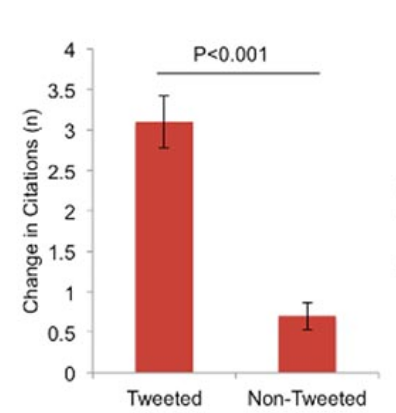
\includegraphics[width=\textwidth]{img/tweet_journal}
    \ppagenote{image from Jessica Luc et al.: \url{https://doi.org/10.1016/h.athoracsur.2020.04.065}}
  \end{columns}

\end{frame}
